\documentclass[PM.tex]{subfiles}
\begin{document}
\chapter{Análisis convexo}
\section{Conjuntos convexos}

\begin{defi}
Un conjunto $S\subseteq\R^n$ es \textbf{convexo} si $\forall x^1,x^2\in S$ y $\forall  \lambda\in[0,1]$ se cumple que $\lambda x^1 + (1-\lambda)x^2\in S$.
\end{defi}

\begin{defi}
Un \textbf{semiespacio} es un conjunto de la forma $H^-=\left\{x\in\R^n: a'x\leq b, a\in\R^n, b\in\R\right\}$ o de la forma $H^+=\left\{x\in\R^n: a'x\geq b, a\in\R^n\,b\in\R\right\}$.
\end{defi}

\begin{prop}
$H^-$ es convexo.
\end{prop}

\begin{dem}
Sea $x(\lambda)\equiv \lambda x^1 + (1-\lambda)x^2, \lambda\in[0,1]$. Se tiene lo siguiente
\[
a'x(\lambda)=a'(\lambda x^1 + (1-\lambda)x^2)=\lambda a'x^1 +(1-\lambda)a'x^2\leq \lambda b+(1-\lambda)b=b
\]
Como queríamos demostrar. $\QED$
\end{dem}

\begin{prop}
Si $S_1$ y $S_2$ son convexos entonces $S_1\cap S_2$ es convexo
\end{prop}
\begin{dem}
Definimos $x(\lambda)$ igual que en la demostración anterior. Supongamos que $S_1$ y $S_2$ tienen intersección no vacía, pues en otro caso el resultado se sigue trivialmente. Dados $x^1,x^2\in S_1 \cap S_2$ se tiene por convexidad de $S_1$ que $x(\lambda)\in S_1$. Análogamente, $x(\lambda)\in S_2$. Por lo tanto, $x(\lambda)\in S_1\cap S_2$. $\QED$
\end{dem}

\begin{defi}
Un \textbf{poliedro} es el conjunto de puntos definido por la intersección de un número finito de semiespacios. Visto matricialmente, dados $A\in\R^{m\times n}, b\in \R^n$ se define el poliedro $P=\left\{x\in \R^n: Ax\leq b\right\}$. Si denotameos por $a_i$ a la i-ésima fila de $A$ vemos que este conjunto se reescribe como $\left\{x\in\R^n: a_ix\leq b_i\ \forall i=1,\dots, n\right\}$, que es equivalente a la primera definición. Un poliedro acotado se llama \textbf{politopo}. 
\end{defi}

\begin{coro}
Los poliedros son convexos.
\end{coro}

\begin{defi}
Se define el \textbf{rayo} por un punto $x\in\R^n$ como el conjunto $\left\{y\in\R^n: y=\lambda x, \lambda\geq 0\right\}$.
\end{defi}

\begin{defi}
Sea S convexo y $x\in S$. El punto $x$ dice \textbf{punto extremo} si $x=\lambda x^1 +(1-\lambda)x^2$ con $x^1,x^2\in S$ y $\lambda\in (0,1)$ implica que $x^1=x^2=x$.
\end{defi}
\begin{nota}  En el caso de los poliedros, los puntos extremos coinciden con la idea de vértice. En una bola euclídea cerrada su frontera es de puntos extremos.
\end{nota}

\begin{defi}
Diremos que $d\in\R^n$ es una \textbf{dirección} de $S\subseteq\R^n$ si $\forall x\in S$ se tiene que $x+\alpha d\in S\ \forall\alpha\geq 0$.
\end{defi}

\begin{defi} Una dirección $d$ es \textbf{extrema} si $d=\alpha^1d^1+\alpha^2d^2$, siendo $d^i$ direcciones de $S$ y $\alpha^1,\alpha^2>0$ implica que $d^1$ es proporcional a $d^2$.
\end{defi}

\begin{defi}
Dados $r$ puntos $x^1,\dots, x^r\in\R^n$ llamamos \textbf{combinación convexa} de estos puntos a $\sum_{i=1}^r\lambda_i x^i$ si $\lambda_i\geq 0\ \forall i=1,\dots, r$ y $\sum_{i=1}^r\lambda_i=1$.
\end{defi}

\section{Teorema de Carathéodory}
\begin{defi} Sean $a^1,\dots, a^d\in\R^n$ afinmente independientes (esto es, que fijado un punto, los vectores diferencia de este con los demás son linealmente independientes). Se denomina \textbf{símplex $(d-1)$-dimensional} a 
\[
S(d-1)= \left\{x\in\R^n:x=\sum_{i=1}^d\lambda_i a^i,\lambda_i\geq 0, \sum_{i=1}^d\lambda_i =1\right\}
\]
\end{defi}
\begin{example}
$S(1)$ es un segmento, $S(2)$ es un triángulo relleno y $S(3)$ es un tetraedro relleno.
\end{example}

\begin{defi} Dado un conjunto $S\subset\R^n$, su \textbf{envolvente} (envoltura) \textbf{convexa} $CO(S)$ es
\[
CO(S)=\left\{x\in\R^n: x=\sum_{i=1}^d\lambda_i x^i, r<+\infty, x^i\in S^1, i=1,\dots, r, \lambda_i\geq 0, \sum_{i=1}^d\lambda_i =1\right\}
\]
$CO(S)$ es el menor convexo que contiene a $S$.
\end{defi}

\begin{defi} Diremos que $C\subset\R^n$ es un cono si contiene a todos sus rayos, es decir, $\forall x\in C$ $\lambda x\in C, \lambda\geq 0$.
\end{defi}
\begin{example}
Una semirrecta que pasa por el origen es un cono. No todos los conos son conjuntos convexos.

\begin{center}
\definecolor{zzttqq}{rgb}{0.6,0.2,0.}
\begin{tikzpicture}[line cap=round,line join=round,>=triangle 45,x=1.0cm,y=1.0cm]
\clip(-3,-2.5) rectangle (3,2.5);
\fill[color=zzttqq,fill=zzttqq,fill opacity=0.10000000149011612] (0.,0.) -- (2.,3.) -- (4.,3.) -- cycle;
\fill[color=zzttqq,fill=zzttqq,fill opacity=0.10000000149011612] (0.,0.) -- (-4.5,-3.) -- (-2.5,-3.) -- cycle;
\fill[color=zzttqq,fill=zzttqq,fill opacity=0.10000000149011612] (0.,0.) -- (4.5,-3.) -- (2.5,-3.) -- cycle;
\draw [color=zzttqq] (0.,0.)-- (2.,3.);
\draw [color=zzttqq] (2.,3.)-- (4.,3.);
\draw [color=zzttqq] (4.,3.)-- (0.,0.);
\draw [color=zzttqq] (0.,0.)-- (-4.5,-3.);
\draw [color=zzttqq] (-4.5,-3.)-- (-2.5,-3.);
\draw [color=zzttqq] (-2.5,-3.)-- (0.,0.);
\draw [color=zzttqq] (0.,0.)-- (4.5,-3.);
\draw [color=zzttqq] (4.5,-3.)-- (2.5,-3.);
\draw [color=zzttqq] (2.5,-3.)-- (0.,0.);
\draw (2.,2.)-- (2.,-2.);
\draw (0.,-4.126140413226097) -- (0.,4.020852846215659);
\draw [domain=-6.367650924229384:10.452891711961001] plot(\x,{(-0.-0.*\x)/2.8572768088505205});
\begin{scriptsize}
\draw [fill=black] (2.,2.) circle (2.5pt);
\draw [fill=black] (2.,-2.) circle (2.5pt);
\end{scriptsize}
\end{tikzpicture}
\end{center}
\end{example}\

\begin{theorem}[Teorema de Carathéodory]
Sea $S\subseteq\R^n$. Si $x\in CO(S)$ entonces:
\[ x = \sum_{i=1}^{n+1} λ_i x^i \]
con $x^i\in S, λ_i ≥ 0$ y $\sum_{i=1}^{n+1}λ_i=1$. Es decir, cualquier punto de la envoltura se puede expresar como combinación lineal convexa de a lo sumo $n+1$ puntos.
\end{theorem}
\begin{dem}
Sea $x \in CO(S)$ y supongamos que:
\[ x = \sum_{i=1}^r λ_i x^i \]
Si $r ≤ n+1$, el teorema está probado. Si $r > n+1$, consideramos los $r-1$ vectores linealmente dependientes $x²-x¹, x³-x¹, \dots, x^{r}-x¹$. Entonces existen $μ_2,\dots,μ_r$ no todos nulos tales que:\[ 0 = \sum_{i=2}^r μ_i (x^i-x¹) = \sum_{i=2}^r μ_i x^i - x^1\sum_{i=2}^r μ_i\]
Tomamos $μ_1 := -\sum_{i=2}^r μ_i$ de manera que se tiene que:
\[ \sum_{i=1}^r μ_i x^i = 0\]
\[ \sum_{i=1}^r μ_i = 0 \]
Sea $α \in \R$. Consideramos:
\[ x = x - α0 = \sum_{i=1}^r λ_i x^i - α \sum_{i=1}^r μ_i x^i = \sum_{i=1}^r (λ_i - α μ_i)x^i \]
Definimos $γ_i = λ_i - α μ_i$ y buscamos $α$ de manera que $γ_i x^i$ sea una combinación convexa. Tomando:
\[ α = \min_{1≤i≤r} \left\{ \frac{λ_i}{μ_i} : μ_i > 0\right\} = \frac{λ_{i*}}{μ_{i*}} \]
Entonces se tiene que $γ_i \geq 0$ y:
\[ \sum_{i=1}^r γ_i = \sum_{i=1}^r (λ_i -α μ_i) = \sum_{i=1}^r λ_i - α \sum_{i=1}^r μ_i = 1 - α \cdot 0 = 1\]
Sin embargo, $γ_{i*} = λ_{i*} - \frac{λ_{i*}}{μ_{i*}}μ_{i*} = 0$, luego $x$ es una combinación convexa de a lo sumo $r-1$ puntos de $S$. Podemos repetir esta construcción hasta llegar a $r = n+1$.
$\QED$
\end{dem}

Consideremos que $||x||$ representa la norma euclídea (se pueden probar resultados análogos con otras normas). 
\begin{theorem}[Teorema de la proyección]
Sea $S\subset\R^n$ convexo y cerrado no vacío, y sea $y\not\in S$ . Entonces existe un único $\overline{x}\in S$ tal que $||y-\overline{x}||=\min_{x\in S}||y-x||$. Además $\overline{x}$ está caracterizado por ser el que verifica $(y-\overline{x})'(x-\overline{x})\leq 0\ \forall x\in S$.

\end{theorem}
\begin{dem}
Supongamos que existe $\overline{x}$: consideramos el conjunto \[ \overline{S}=S\cap\{x\in\R^n : ||y-x||\leq ||y-x^0||\}\] para cualquier $x^0\in S$ fijo. Entonces $\inf_{x\in S}||y-x||=\inf_{x\in\overline{S}}||y-x||$. Además, $\overline{S}$ es cerrado y acotado, por tanto el teorema de Weierstrass asegura que existe el $\min_{x\in\overline{S}}||y-x||$ que será $\overline{x}$. Veamos que es único. Supongamos que existe otro $\hat{x}\in S$ tal que 
\[
\gamma=||y-\hat{x}||=||y-\overline{x}||=\min_{x\in\overline{S}}||y-x||
\]
Consideramos el punto medio $\dfrac{\overline{x}+\hat{x}}{2}\in S$ por ser $S$ convexo. Ahora, aplicando la desigualdad triangular
\[
|| y-\frac{\overline{x}-\hat{x}}{2}||=||\frac{y}{2}-\frac{\overline{x}}{2}+\frac{y}{2}-\frac{\hat{x}}{2}||\leq ||\frac{y-\overline{x}}{2}||+||\frac{y-\hat{x}}{2}||=\frac{1}{2}\left(||y-\overline{x}||+||y-\hat{x}||\right)
\]
Como $\gamma$ era la distancia mínima, las desigualdades en realidad son igualdades. La desigualdad triangular solo se convierte en igualdad cuando los vectores son proporcionales, luego $y-\overline{x}=\alpha(y-\hat{x})$, y como ambos tienen norma $\gamma$, necesariamente $|\alpha|=1$. Si $\alpha=-1$ entonces $y-\overline{x}=-(y-\hat{x})\Rightarrow 2y=\hat{x}+\overline{x}\Rightarrow y=\dfrac{\hat{x}+\overline{x}}{2}\in S$, lo cual no es posible porque habíamos supuesto que $y\not\in S$. Por lo tanto $\alpha=1$ y deducimos que $\overline{x}=\hat{x}$.\\
Por último probemos la caracterización. Supongamos que $\overline{x}$ verifica $(y-\overline{x})'(x-\overline{x})\leq 0\ \forall x\in S$. Entonces $\forall x\in S$
\[
||y-x||^2=||y-\overline{x}+\overline{x}-x||^2=||y-\overline{x}||^2+||\overline{x}-x||^2+2(y-\overline{x})'(\overline{x}-x)
\]
El último término es mayor o igual que $0$ por hipótesis, y como la norma es siempre no negativa deducimos que $||y-x||\leq ||y-\overline{x}||^2\ \forall x\in S$. Recíprocamente, supongamos que $\overline{x}$ es el mínimo.  Consideramos entonces para cada $x\in S$ el punto $\overline{x}+\lambda(x-\overline{x})$ con $\lambda\in (0,1)$. Entonces, 
\[
||y-(\overline{x}+\lambda(x-\overline{x}))||^2=||y-\overline{x}||^2+\lambda^2||\overline{x}-x||-2\lambda(y-\overline{x})'(x-\overline{x})\geq||y-\overline{x}||.
\]
Para que sea posible esa desigualdad, necesariamente $\lambda^2||\overline{x}-x||-2\lambda(y-\overline{x})'(x-\overline{x})\geq 0$. Simplificamos y despejamos y tenemos que $\lambda||x-\overline{x}||\geq 2\lambda(y-\overline{x})'(x-\overline{x})$. Como vale para todo $\lambda\in (0,1)$, en particular vale para el límite ($\lambda=0$), luego $0\geq (y-\overline{x})'(x-\overline{x})$. $\QED$
\end{dem}

\begin{defi} Sean dos conjuntos convexos $S_1,S_2\subset\R^n$ y el hiperplano $H=\{x\in\R^n: p'x=\alpha\}$. Decimos que $H$ separa $S_1$ de $S_2$ si $p'x\leq\alpha \forall x\in S_1$ y $p'x\geq\alpha \forall x\in S_2$. Se dice que $H$ separa estrictamente a $S_1$ de $S_2$ si las desigualdades son estrictas.
\end{defi}

\begin{lema}
Sea $S\subset\R^n$ convexo y cerrado, sea $y\not\in S$. Existen $p\in\R^n, \alpha\in\R$ tal que $p'y<\alpha$ y $p'x\leq\alpha\ \forall x\in S$.
\end{lema}
\begin{dem}
Por el teorema de la proyección, existe $\overline{n}\in S$ tal que $(y-\overline{x})'(x-\overline{x})\leq 0\ \forall x\in S$. Tomamos $p=(y-\overline{x})$ y $\alpha=p' \overline{x}$. Luego $p'(x-\overline{x})\leq 0\equiv p'x\leq p'\overline{x}$. Además, como $y\not\in S$, $0<||y-\overline{x}||^2=(y-\overline{x})'(y-\overline{x})=p'y-\underbrace{p'\overline{x}}_\alpha \Rightarrow \alpha <p'y$. $\QED$
\end{dem}

\newpage

\begin{lema}[de Farkas]
Sean $A\in \R^{m\times n}, b\in\R^m,x\in\R^n$. Entonces, exactamente uno de los siguientes sistemas tiene solución:
\begin{enumerate}
\item $Ax=b$ con $x\geq 0$ (es decir, todas las componentes de $x$ son no negativas).
\item $u'A\leq 0, u'b>0, u\in R^m$.
\end{enumerate}
\end{lema}

Antes de demostrarlo vamos a interpretarlo. Sean $a_1,\dots, a_n$ las columnas de $A$. Entonces $Ax=a_1x_1+\cdots +a_nx_n$ con $x_i\geq 0\ \forall i$. Las combinaciones no negativas de los vectores $a_i$ generan un cono. Del segundo sistema $u'a_1\leq 0,\dots , u'a_n\leq 0$. Luego el ángulo que forma $u'$ con cada $a_i$ es mayor de $\frac{\pi}{2}$ y $u$ está en la intersección de todos los hiperplanos. Por otro lado $b$ tiene que formar un ángulo con $u$ menor de $\frac{\pi}{2}$ por lo que estará fuera del cono. Por tanto, si el segundo sistema tiene solución, el primero no puede tenerlo porque en el primero $b$ debe estar dentro del cono. Ver figura.

\begin{dem}\
\begin{enumerate}
\item Supongamos que el primer sistema tiene solución. Es decir, $\exists x^0\mid Ax^0=b, x^0\geq 0$. Por tanto $u'A\cdot x^0\leq 0\equiv u'b\leq 0$, luego no puede haber solución en el segundo.
\item Supongamos que el primer sistema no tiene solución. El conjunto $S=\{v: v=Ax,x\geq 0\}$ es convexo y cerrado en $\R^m$ y $b\not\in S$. Aplicando el mea anterior existen $p\in\R^m,\alpha\in\R$ tal que $p'b>\alpha, p'v\leq\alpha\ \forall v\in S$. Como $0\in S$ deducimos que $p'0\leq\alpha$ luego $\alpha\geq 0$ y por tanto $p'b>\alpha\geq 0\Rightarrow p'b>0$. Ahora tenemos que probar que $p'A\leq 0$. Utilizamos que $p'v\leq\alpha\ \forall v\in S$. Entonces $p'Ax\leq\alpha\ \forall x\geq 0$. De aquí deducimos que todas las componentes de $p'A$ deben ser no positivas, porque si hubiera una componente positiva (supongamos que es la $i$-ésima) entonces $(p'A)_ix_i>0$. Tomando $x_i\rightarrow +\infty$ se tiene que $(p'A)_i\rightarrow +\infty$, por lo que será mayor que $\alpha$.
\[
(p'Ax)=\sum_{j\neq i}(p'A)_jx_j + (p'A)_ix_i \rightarrow +\infty.
\]
Por tanto  $p'Ax\leq\alpha$ y hemos encontrado una solución para el segundo sistema.
\end{enumerate}
\end{dem}

\begin{coro}
Los siguientes sistemas son alternativos:
\begin{enumerate}
\item $Ax\geq b, x\geq 0$.
\item $u'A\leq 0, u\geq 0, u'b>0$. 
\end{enumerate}
\end{coro}
\begin{dem}
\begin{enumerate}
\item Denotamos por $A_i$ la fila $i$ de $A$ con $i\in\{1,\dots,m\}$. Entonces 
\[
Ax\geq b, x\geq 0 \equiv\begin{cases}
A_1x\geq b_1\equiv A_1x-y_1 & y_1\geq 0\\
\vdots & \\
A_mx\geq b_m\equiv A_mx-y_m & y_m\geq 0\\
x\geq 0 & 
\end{cases}
\]
es decir, $Ax\geq b, x\geq 0 \equiv Ax-Iy=b, x\geq 0, y\geq 0$, o lo que es lo mismo,
\[(A| -I)\begin{pmatrix}
x\\
y
\end{pmatrix}=b\quad x,y\geq 0.
\]
Ya lo tenemos expresado como el lema de Farkas. Su alternativa es 
\item $u'(A| -I)\leq 0, u'b>0$, es decir, $u'A\leq 0, u'(-I)\leq 0, u'b>0 \Leftrightarrow u'A\leq 0, u\geq 0, u'b>0$. $\QED$
\end{enumerate}
\end{dem}

\begin{lema}
Sea $K\in\R^{n\times m}$ tal que $K'=-K$. Entonces, el sistema $Kx\geq 0, x\geq 0$ tiene una solución que verifica $Kx+x>0$.
\end{lema}
\begin{dem}
Vamos a aplicar el corolario con $b=e_i$ (el vector columna nulo salvo la componente $i$-ésima, que vale $1$), $i=1,\dots, n$.
Consideramos el sistema $Kx\geq e_i, x\geq 0$ o su alternativa $x'K\leq 0, x\geq 0, x'e_i>0$. Sea $\overline{x}^i$ las solución de este par de sistemas en alternativa (es decir, que es solución de uno o de otro). Si $\overline{x}^i$ es solución del primero:
\[
\begin{cases}
K_i\overline{x}^i\geq 1 & \\
K_j\overline{x}^j\geq 0 & j\neq i\\
\overline{x}^i\geq 0 &
\end{cases}
\]
por lo que $K_i\overline{x}^i+\overline{x}^i>0$ y $ K_i\overline{x}^i_i + \overline{x}^i_j\geq 0\ \forall j\neq i$. Por el contrario, si $\overline{x}^i $ es solución del segundo sistema llegamos a que $K'\overline{x}^i\leq 0, \overline{x}^i\geq 0, e'_i\overline{x}^i>0$ y usando que $K$ es antisimétrica obtenemos $K\overline{x}^i\geq 0, e'_i\overline{x}^i>0$. De la última desigualdad deducimos que $\overline{x}^i_i> 0\ \forall i$. Por tanto
\[
K_i\overline{x}^i_i +\overline{x}^i_i>0\quad K_j\overline{x}^i_j +\overline{x}^i_j\geq 0\ \forall j\neq i.
\]
En ambos casos obtenemos lo mismo. Consideramos $\overline{x}=\sum_{i=1}^n\overline{x}^i$. Cumple que $K\overline{x}\geq 0, \overline{x}\geq 0$. Además, 
\[
K\overline{x}+\overline{x}=K(\sum_{i=1}^n\overline{x}^i)+\sum\overline{x}=\sum_{i=1}^n(K\overline{x}^i+\overline{x}^i)>0
\]
$\QED$
\end{dem}

\section{Representación de poliedros}

\begin{defi}
Diremos que un poliedro $P$ está en forma estándar si $P=\{x\in\R^n: Ax=b,x\geq 0\}$ con $A\in\R^{m\times n}, b\in\R^m, b\in\R^m, n\geq m$ y $rg(A)=m$.
\end{defi} 
\begin{nota}
Todo poliedro se puede escribir en forma estándar pues $a'x\leq b\equiv a'x+y=b, y\geq 0$ y análogamente restando para la desigualdad contraria.
Si $x_j\in\R$ entonces podemos escribir $x_j=x_j^+ -x_j^-$ siendo $x_j^+=\max{\{x_j,0\}}, x_j^-=-\min{\{x_j,0\}}$.
\end{nota}

Dado que $A\in\R^{m\times n}, b\in\R^m, n\geq m$ y $rg(A)=m$, existe una matriz $B$ de $m$ columas de $A$ que son linealmente independientes, es decir que $rg(B)=m$ ($\exists B^{-1}$). Escribimos entonces $A$ como $[B\ N]$ poniendo las columnas independientes al principio. Las variables del sistema $Ax=b$ también se deben reordenar de modo que 
\[
Ax=b\equiv [B\ N]\begin{bmatrix}
x_B\\
x_N
\end{bmatrix}=b
\]

Sea $A \subset \R^{m \times n}$, $rg(A) = m$, $m ≤ n$ y $b \in \R^m$. Consideramos $P = \{ x \in \R^n : Ax=b, x ≥ 0\}$ (poliedro en forma estándar).

\begin{theorem}[Teorema de caracterización de puntos extremos]\label{carac-extremos}
Se $P$ un poliedro en las condiciones anteriores. Entonces $x$ es un punto extremo de $P$ si y sólo si existe $B \subset A$ con $B \in \R^{m \times m}$, $rg(B)=m$, $B^{-1}b ≥ 0$ y $x = \begin{pmatrix} B^{-1}b\\0\end{pmatrix}$
\end{theorem}

\begin{dem}
($\Leftarrow$) Supongamos que $x =\begin{pmatrix} B^{-1}b\\0\end{pmatrix}$, $B \subset A$ con $B \in \R^{m \times m}$, $rg(B)=m$, $B^{-1}b ≥ 0$. Usaremos reducción al absurdo, supongamos que existe $x^1$, $x^2 \in P$ tal que $x = λx^1+(1-λ)x^2$ con $λ \in (0,1)$. Tenemos que $A = [B\ N]$ y $x = \begin{pmatrix}x_B\\x_N\end{pmatrix} = \begin{pmatrix} B^{-1}b\\0\end{pmatrix}$, $x^1 = \begin{pmatrix}x_B^1\\x_N^1\end{pmatrix}$ y $x^2 = \begin{pmatrix}x_B^2\\x_N^2\end{pmatrix}$ Luego:
\[ x = \begin{pmatrix} B^{-1}b\\0\end{pmatrix} = λ\begin{pmatrix}x_B^1\\x_N^1\end{pmatrix}+(1-λ)\begin{pmatrix}x_B^2\\x_N^2\end{pmatrix} \]
De ahí, $0 = λ x_N^1 + (1-λ) x_N^2$. Como $x_N^i ≥ 0$, se sigue que $x_N^i = 0$. De $x^i \in P$, se sigue que $Ax^i = b \equiv [B\ N]\begin{bmatrix}x_B^i\\0
\end{bmatrix} = b \equiv Bx_B^i + N0 = b$. Por lo tanto: $x_B^i = B^{-1}b \geq 0$, luego $x^i = \begin{pmatrix}B^{-1}b\\0\end{pmatrix}=x$ para $i=1,2$.

($\Rightarrow$) Supongamos que $x$ fuera un punto extremo de $P$. Se tiene que $Ax=b, x ≥ 0$. Como $rg(A) = m$ podemos suponer sin pérdida de generalidad que $x^1 =(x_1,\dots,x_k,0,\dots,0)$ con $x_i > 0$ y $k ≤ m$.
Vamos a probar que las columnas asociadas a estas coordenadas $(a_1, a_2, \dots, a_k)$ son linealmente independientes. Si no lo fueran, existirían $λ_1,λ_2, \dots, λ_k$ tales que $\sum_{i=1}^k λ_i a_i = 0$. Denotamos or $λ' =(λ_1,\dots,λ_k,0,\dots,0)$. Entonces $Aλ=λ_1a_1 + λ_2a_2 + \cdots + λ_ka_k + 0a_{k+1}+\cdots+0a_n = 0$. Entonces podemos considerar los puntos $x^1 = x+αλ$ y $x^2 = x-αλ$ y $α > 0$. Claramente $x^1 \neq x^2$ y $x = \frac{1}{2}x^1+ \frac{1}{2}x^2$. Veamos que $x^i \in P$ para $i=1,2$.
\[ Ax^i = A(x + αλ) = Ax + α(\underset{=0}{Aλ}) = Ax = b \]
\[ x^i = x \pm αλ = \begin{pmatrix}x_1\\\vdots\\x_k\\0\\\vdots\\0\end{pmatrix} + α \begin{pmatrix}λ_1\\\vdots\\λ_k\\0\\\vdots\\0\end{pmatrix} \]
Por hipótesis, $x_1,\dots,x_k > 0$. Tomando $α$ suficientemente pequeño, podemos asegurar que $x_i \pm αλ_i > 0$. Entonces $x^i \geq 0$ y $x^i \in P$. Esto contradice que $x$ sea un punto extremo. Podemos entonces asegurar que $(a_1,\dots,a_k)$ son linealmente independientes. Podemos completar $(a_1,\dots,a_m)$ hasta $m$ columnas linealmente independientes (podemos ya que $rg(A) = m$). Tomamos $B = (a_1,\dots,a_m)$. Entonces:
\[ Ax =[B\ N]\begin{pmatrix}x_1\\\vdots\\x_k\\0\\\vdots\\0\end{pmatrix}_{(n)} = B \begin{pmatrix}x_1\\\vdots\\x_k\\0\\\vdots\\0\end{pmatrix}_{(m)} +N0_{(m-n)} = b \]
Luego: \[ \begin{pmatrix}x_1\\\vdots\\x_k\\0\\\vdots\\0\end{pmatrix} = B^{-1}b \geq 0 \qquad x = \begin{pmatrix}B^{-1}b\\0\end{pmatrix} \]
\end{dem}

\begin{nota}
El número de puntos extremos de los poliedro es finito y está acotado por el número combinatorio $\begin{pmatrix}n\\m\end{pmatrix}$.
\end{nota}

\begin{lema}
$d$ es una dirección de $P$ si y sólo si $Ad=0$, $d ≥ 0$.
\end{lema}

\begin{dem}
$d$ es dirección sii $\forall x \in P$, $x + λd \in P$ $\forall λ ≥ 0$. Equivalentemente, $A(x+λd)= b$ y $x+λd ≥ 0$ $\forall λ ≥ 0$. Esto se cumple sii:
\[ Ax+λAd = b \Leftrightarrow Ad = 0\]
\[ x + λd ≥ 0 \forall λ ≥ 0 \Leftrightarrow d ≥ 0 \]
\end{dem}

\begin{theorem}[Teorema de caracterización de direcciones extremas]\label{carac-direcciones}
$d$ es una dirección extrema de $P$ sii $d = \begin{pmatrix}-B^{-1}a_j\\e_j\end{pmatrix}$ donde $B \subset A$, $B \in R^{m\times m}$, $rg(B) = m$ y $a_j \notin B$ tal qe $B^{-1}a_j ≤ 0$. (Demostrado en uno de los libros de Bazaraa)
\end{theorem}

\begin{nota} El número de direcciones extremas de $P$ es finito y está acotado por $\begin{pmatrix}n\\m\end{pmatrix}(n-m)$.
\end{nota}

\begin{theorem}[Teorema de representación de poliedros de Minkowski-Weyl]
Sea $P$ un poliedro en forma estándar y sean $x^1,x²,\dots,x^k$ sus puntos extremos y $d^1,d^2,\dots,d^l$ sus direcciones extremas. Consideramos 
\[ S = \{x \in \R^n : x = \sum_{i=1}^k λ_i x^i + \sum_{j=1}^l μ_j d^j, \sum_{i=1}^k λ_i=1, λ_i ≥ 0, μ_j ≥ 0\ \forall i,j\} \]
Entonces $S = P$. Es decir, cualquier poliedro en forma estándar queda determinado por sus extremos y direcciones extremas.
\end{theorem}

\begin{dem} Lo demostraremos por doble inclusión:
\begin{itemize}
	\item $(S \subseteq P)$ Sea $x \in S$, $x = \sum_{i=1}^k λ_i x^i + \sum_{j=1}^l μ_j d^j$ para algún $λ$ y $μ$.
	\[ Ax = A\left( \sum_{i=1}^k λ_i x^i + \sum_{j=1}^l μ_j d^j\right) =  \sum_{i=1}^k \underset{=b}{λ_i x^i} + \sum_{j=1}^l μ_j \underset{=0}{Ad^j} = \sum_{j=1}^l b = b \]
	\[ x = \sum_{i=1}^k \underset{≥0}{λ_i} \underset{≥0}{x^i} + \sum_{j=1}^l \underset{≥0}{μ_j}\underset{≥0}{d^j} ≥ 0 \]
	Luego $x \in P$
	
	\item $(P \subseteq S)$ Supongamos que existe $z \in P$ pero $z \notin S$. Como $S$ es un convexo cerrado, existe $p \in \R^n$, $α \in \R$ tales que $p'z > α$, $p'x ≤ α$ $\forall x$ (separación de $z$ y $S$). Tenemos
	\begin{enumerate}
		\item $p'd^j ≤ 0$ $\forall j=1,\dots,l$
		
		Si existiese $j$ tal que $p'd^j > 0$, consideamos el rayo $x + λd^j, λ ≥ 0$ para cualquier $x \in S$, pero entonces $p'(x+λd^j) = p'x + λp'd^j ≤ α$, pero $λp'd^j$ tiende a infinito cuando $λ$ tiende a infinito, luego $p'(x+λd^j)$ no puede estar acotado por ningún $α$.
		\item $p'z > α ≥ p'x^i$ $\forall i=1,\dots,k$
	\end{enumerate}
	Sea $\overline{x}$ el punto extremo tal que $p'\overline{x} = \max_i p'x^i$. Usando el teorema \ref{carac-extremos}: existe una reordenación tal que $\overline{x} = \begin{pmatrix}B^{-1}b\\0\end{pmatrix}$, $A = [B\ N]$, $x = \begin{bmatrix}x_B\\x_n\end{bmatrix}$, $z = \begin{bmatrix}z_B\\z_n\end{bmatrix} \in P$, $Az=b$. De $[B\ N]\begin{bmatrix}z_B\\z_N\end{bmatrix} = b$ obtenemos que $z_B = B^{-1}b-B^{-1}Nz_N$. Luego usando (2):
	\[ 0 < p'(z-\overline{x}) = (p_B'\ p_N') \left[\begin{pmatrix}B^{-1}b-B^{-1}Nz_N\\z_N\end{pmatrix}-\begin{pmatrix}B^{-1}b\\0\end{pmatrix}\right] =-p_B'B^{-1}Nz_N + p'z_N = (p_N'-p_B'B^{-1}N)z_N \]
	Al menos una de las coordenadas de $p_N'-p_B'B^{-1}N$ debe ser positiva. Sea $j$ tal que:
	\[ 0 < (p_N'-P_B'B^{-1}N)_j = p_j - p_B'B^{-1}a_j \]
	Llamemos $y_j\footnote{\url{https://www.youtube.com/watch?v=q6EoRBvdVPQ}} = B^{-1}a_j$ . Veamos que $y_j > 0$. Si $y_j ≤ 0$, $d = \begin{pmatrix}-B^{-1}a_j\\e_j\end{pmatrix}$ debe ser una dirección extrema por el teorema \ref{carac-direcciones}. Entonces $p'd = (p_B'\ p_N')\begin{pmatrix}-B^{-1}a_j\\e_j\end{pmatrix}=-p_B'B^{-1}a_j + p_j > 0$, pero esto contradice (1). Luego $y_j = B^{-1}a_j > 0$. Denotemos por $\overline{b}=B^{-1}b$. Sea $d = \begin{pmatrix}-y_j\\e_j\end{pmatrix}$ y $\hat{x} = \overline{x} + λd$. Veamos que $\hat{x} \in P$ si $λ = \frac{\overline{b}_r}{y_{jr}} = \min\{\frac{\overline{b}_i}{y_{ji}} : y_{ji} > 0\}$..
	\[ A\hat{x} = A\overline{x} + \frac{\overline{b}_r}{y_{r_j}} A d = b + \frac{\overline{b}_r}{y_{jr}} [B\ N] \begin{pmatrix}-B^{-1}a_j\\e_j\end{pmatrix} = b + \frac{\overline{b}_r}{y_{jr}}(-a_j + a_j) = b \]
	Si $i$ es una cooredanda de $B$ con $i \neq r$:
	\[ \hat{x}_i = (B^{-1}b)_i + \frac{\overline{b}_r}{y_{jr}}(-y_{ji}) = \overline{b}_i - \frac{\overline{b}_r}{y_{jr}}y_{ji} \]
	Si $y_{ji} < 0 \Rightarrow \hat{x} ≥ 0$ evidentemente. Si $y_{ji} > 0$, entonces $\overline{b}_i - \frac{\overline{b}_r}{y_{jr}}y_{ji} ≥ 0$, ya que $ \frac{\overline{b}_r}{y_{ji}} ≥ \frac{\overline{b}_r}{y_{jr}}$.
	
	Si $i = r$, el resultado es directo, ya que $\overline{b}_r - \frac{\overline{b}_r}{y_{jr}}y_{jr} = 0 ≥ 0$.
	
	Si $i$ es una coordenada que está en $N$, se tiene que $i \neq j$, luego:
	\[ \hat{x}_i = 0 +  \frac{\overline{b}_r}{y_{jr}}0 = 0 \]
	\[ \hat{x}_j = 0 +  \frac{\overline{b}_r}{y_{jr}}1 ≥ 0 \]
	
	Luego $\hat{x} \in P$. Además $\hat{x}$ es un punto extremo representado por las columnas $\hat{B}= (a_1,\dots,a_m)$ y además verifica:
	\[ p'\hat{x} = p'(\overline{x} + \frac{\overline{b}_r}{y_{jr}}d) = p'\overline{x} + \underset{>0}{\frac{\overline{b}_r}{y_{jr}}} \underset{≥0}{p'd} > p'\overline{x} \]
	Esto contradice que $p'\overline{x}$ fuera máximo. Por reducción al absurdo, llegamos a que $z \in S$, lo que acaba la demostración.
	$\QED$
\end{itemize}
\end{dem}

\chapter{Programación Lineal} %Debería ser capítulo 3

\section{Resolución de problemas de Programación Lineal}

Sean $A\in\R^{m\times n},\ rg(A)=m,\ m\leq n,\ b\in\R^m,\ c\in\R^n$. Consideramos el poliedro en forma estándar $P=\{x\in\R^n: Ax=b\}$. El problema de programación lineal consiste en $\underset{x\in P}{\min} c'x \equiv \underset{Ax=b,x\geq 0}{\min} c'x\equiv (PL)$. 

\begin{theorem}[Teorema fundamental de la PL] Supongamos que $x^1,\dots ,x^k$ y $d^1,\dots ,d^l$ son respectivamente los puntos extremos y direcciones extremas de $P$. Entonces, la condición necesaria y suficiente para que $(PL)$ tenga solución óptima es que $c'd^j\geq 0\ \forall j=1,\dots, l$. En este caso, una solución óptima siempre se alcanza en un vértice de $P$.
\end{theorem}
\begin{dem}
Planteamos el problema de programación lineal $\underset{Ax=b,x\geq 0}{\min} c'x$. Por el teorema de Wein, si $x\in P$, podemos escribir $x=\sum_{i=1}^k\lambda_ix^i +\sum_{j=1}^l\mu_j d^j$ con $\lambda_i\geq 0, \mu_j\geq 0, \sum_{i=1}^k\lambda_i=1$. Luego tenemos el problema siguiente
\[\underset{\lambda_i\geq 0, \mu_j\geq 0, \sum_{i=1}^k\lambda_i=1}{\min} c'[\sum_{i=1}^k\lambda_ix^i +\sum_{j=1}^l\mu_j d^j] \]
Supongamos que $c'd^j\geq 0\\forall j$. Entonces continuamos la ecuación anterior con 
\begin{gather*}
 \underset{\lambda_i\geq 0, \mu_j\geq 0, \sum_{i=1}^k\lambda_i=1}{\min} [\sum_{i=1}^n\lambda_ic'x^i +\sum_{j=1}^l\mu_j \underset{\geq 0}{c'd^j}]\geq\\
\underset{\lambda_i\geq 0, \mu_j\geq 0, \sum_{i=1}^k\lambda_i=1}{\min} [\sum_{i=1}^n\lambda_ic'x^i]\geq \\
\underset{\lambda_i\geq 0, \mu_j\geq 0, \sum_{i=1}^k\lambda_i=1}{\min} [\sum_{i=1}^n\lambda_ic'\overline{x}]=\\
\underset{\lambda_i\geq 0, \mu_j\geq 0, \sum_{i=1}^k\lambda_i=1}{\min} [c'\overline{x}\sum_{i=1}^n\lambda_i]=c'\overline{x}
\end{gather*}
donde $\overline{x}$ minimiza $c'x^i$. Como $\overline{x}$ es un punto extremo, $c'x$ es el valor mínimo, entonces $\overline{x}\in P$. Recíprocamente, si $\exists j\mid c'd^j<0$ consideramos $x\in P$ y el rayo $x+\lambda d^j\in P\ \forall\lambda\geq 0$. 
\[ c'(x+\lambda d^j)=\underset{cte}{c'x} + \underset{<0}{\lambda c' d^j}\underset{\lambda\to\infty}{\longrightarrow} -\infty\]
\end{dem}

\begin{nota}
Dada una función $f$ que alcanza un mínimo en $S\subset\R^n$, entonces \[\min_{x\in S} f(x)= -\max_{x\in S}-f(x)\].
\end{nota}


Supongamos que $\overline{x}$ es un punto extremo de $P$ representado por $B\subset A, rg(B)=m, B^{-1}b\geq 0$. Es decir, $\overline{x}=\begin{pmatrix}
B^{-1}b\\
0
\end{pmatrix}$. Reordenamos las columnas de la forma $A=(B N)$. Sea $x\in P$ otro punto genérico. Entonces $x\begin{pmatrix}
x_B\\
x_N
\end{pmatrix}$. Como $Ax=b, x\geq 0$ entonces
\[ (B N) \begin{pmatrix}
x_B\\
x_N
\end{pmatrix}= b\equiv Bx_B + Nx_N=b\].
Luego $x_B=B^{-1}b-B^{-1}Nx_N$, así que 
\[ x=\begin{pmatrix}
B^{-1}b-B^{-1}Nx_N\\
x_N
\end{pmatrix}\]
Ahora bien, $c'x=(c'_B, c'_N)\begin{pmatrix}
B^{-1}b-B^{-1}Nx_N\\
x_N
\end{pmatrix}=\underbrace{c'_B B^{-1}b}_{c'\overline{x}}-c'_N B^{-1}Nx_N=c'\overline{x}+(c'_N-c'_BB^{-1}N)x_N$. Si $c'_N-c'_BB^{-1}N\geq 0$, entonces $c'x\geq c'\overline{x}$, por lo que $\overline{x}$ es mínimo. Si esta condición no se cumple, existirá $j$ tal que $a_j\in N$ de forma que $c_j-c'_BB^{-1}a_j<0$. Construimos $d_j=\begin{pmatrix}
-B^{-1}a_j\\
e_j
\end{pmatrix}$ y consideramos $\overline{x}+\lambda d_j,\ \lambda\geq 0$. La evaluación de $x(\lambda)$ será 
\begin{gather*}
c'x(\lambda)=c'(\overline{x}+\lambda d_j)=c'\overline{x}+\lambda c'd_j=c'\overline{x}+\lambda(c'_B, c'_N)\begin{pmatrix}
-B^{-1}a_j\\
e_j
\end{pmatrix}=\\
c'\overline{x}+\lambda\underbrace{(-c'_B B^{-1}a_j +c_j)}_{<0}< c'\overline{x}, \forall\lambda >0.
\end{gather*}
Es decir, $c'x(\lambda)<c'\overline{x}, \forall\lambda >0$. Si $B^{-1}a_j\leq 0$, por el teorema de representación de direcciones extremas, $d_j$ será una dirección de $P$. Por ello, toda la semirrecta $x(\lambda)=\overline{x}+\lambda d_j\subset P$, es decir, $x(\lambda)\in P\forall\lambda >0$. Entonces $c'x(\lambda)\underset{\lambda\to\infty}{\longrightarrow} -\infty$, esto es, no existe mínimo.

En otro caso, $B^{-1}a_j\not\leq 0$. Denotamos $y_j=B^{-1}a_j, \overline{b}=B^{-1}b$. Esto es, $\exists i\mid y_{ij}>0$. Entonces puedo considerar 
\[
\frac{\overline{b}_r}{y_{rj}}=\min\{\frac{\overline{b}_i}{y_{ij}}:y_{ij}>0\}
\]
y el punto $x(\frac{\overline{b}_r}{y_{rj}})=\overline{x}+\frac{\overline{b}_r}{y_{rj}}d_j$. Vamos a probar que $x(\frac{\overline{b}_r}{y_{rj}})\in P$.
\begin{itemize}
\item $x(\frac{\overline{b}_r}{y_{rj}})\geq 0$. Sea $d_j=\begin{pmatrix}
-y_j\\
e_j
\end{pmatrix}$ Si $i\in B, i\neq r$, $\overline{b}_i-\frac{\overline{b}_r}{y_{rj}}y_{ij}\geq 0$ si y solo si $\frac{\overline{b}_i}{y_{ij}}\geq\frac{\overline{b}_r}{y_{rj}}$ si $y_{ij}>0$, lo cual es cierto por definición. Si $y_{ij}<0$ entonces $\overline{b}_i-\frac{\overline{b}_r}{y_{rj}}y_{ij}\geq 0$.\\
Si $r\in B$, $\overline{b}_r-\frac{\overline{b}_r}{y_{rj}}y_{rj}=0$.\\
Si $i\in N, i\neq j$, entonces $\overline{x}_i+\frac{\overline{b}_r}{y_{rj}}d_{ij}$.\\
Si $j\in N$, entonces $\overline{x}_j+\frac{\overline{b}_r}{y_{rj}}d_{ij}=0+\frac{\overline{b}_r}{y_{rj}}\cdot 1=\frac{\overline{b}_r}{y_{rj}}>0$.

\item $Ax(\frac{\overline{b}_r}{y_{rj}})=b$. Comprobémoslo. $Ax(\frac{\overline{b}_r}{y_{rj}})=[B N]\left[\begin{pmatrix}
B^{-1}b\\
0
\end{pmatrix}+\frac{\overline{b}_r}{y_{rj}}\begin{pmatrix}
-B^{-1}a_j\\
e_j
\end{pmatrix}\right]=b+\frac{\overline{b}_r}{y_{rj}}(-a_j+a_j)=b$.
\end{itemize}
En definitiva $x(\frac{\overline{b}_r}{y_{rj}})\in P$ y es un punto extremo con $\hat{B}=B\setminus\{a_r\}\cup\{a_j\}$. Evitando el ciclado (dos soluciones iguales, de forma que alterna de una a otra) este algoritmo encuentra la solución en un número finito de pasos.

\begin{example}
\begin{align*}
\min &x_1-3x_2\\
sa & -x_1+2x_2\leq 6\\
   & x_1+x_2\leq 5\\
   &x_1,x_2\geq 0
\end{align*}
Para pasarlo a forma estándar sumamos variables (inmersión de $\R^2$ en $\R^4$).
\begin{align*}
\min &x_1-3x_2+0x_3+0x_4\\
sa & -x_1+2x_2+x_3 \quad = 6\\
   & x_1+x_2 \qquad +x_4 = 5\\
   &x_1,x_2,x_3,x_4\geq 0
\end{align*} %alinearlo para que quede todo en su sitio
Entonces $c'=[1,-3,0,0]$, $b=\begin{bmatrix}
6\\
5
\end{bmatrix}$, $A=\begin{bmatrix}
-1 & 2 & 1 0\\
1 & 1 & 0 & 1
\end{bmatrix}$. Elegimos las dos últimas columnas de $A$ para construir $B=[a_3\ a_4]$, que tiene inversa. Además cumple que $B^{-1}b=b\geq 0$. El punto es
\[
\begin{bmatrix}
x_3\\
x_4\\
x_1\\
x_2
\end{bmatrix}=\begin{bmatrix}
B^{-1}b\\
0
\end{bmatrix}=\begin{bmatrix}
6\\
5\\
0\\
0
\end{bmatrix}\]
Comprobamos la condición de optimalidad $c'_N-c'_B B^{-1}N\geq 0$. 
\[
[1,-3]-[0,0]I\begin{bmatrix}
-1 & 2\\
1 & 1
\end{bmatrix}=[1,-3]
\]
El coeficiente negativo corresponde a $a_2$. Calculamos $y_2=B^{-1}a_2=I\begin{bmatrix}
2\\
1
\end{bmatrix}\not\leq 0$. Por lo que tenemos que calcular $\min\{\frac{\overline{b}_i}{y_{i2}}:y_{i2}>0\}=\min\{\frac{6}{3},\frac{5}{1}\}=2$. Como este mínimo corresponde al primer elemento del conjunto, se corresponde con la primera columna de $B$, es decir, $a_3$. Por ello, construimos una nueva $B=[a_2\ a_4]=\begin{bmatrix}
2 & 0\\
1 & 1
\end{bmatrix}$ y $B^{-1}=\begin{bmatrix}
\frac{1}{2} & 0\\
-\frac{1}{2} & 1
\end{bmatrix}$. Por tanto $\overline{b}=B^{-1}b=\begin{bmatrix}
3\\
2
\end{bmatrix}\geq 0$. Así pues $\hat{x}=\begin{bmatrix}
x_2\\
x_4\\
x_1\\
x_3
\end{bmatrix}=\begin{bmatrix}
3\\
2\\
0\\
0
\end{bmatrix}$ Ahora, con $N=\begin{bmatrix}
-1 & 1\\
1 & 0
\end{bmatrix}$, $c'_N-c'_B B^{-1}N=[1,0]-[3,0]\begin{bmatrix}
\frac{1}{2} & 0\\
-\frac{1}{2} & 1
\end{bmatrix}\begin{bmatrix}
-1 & 1\\
1 & 0
\end{bmatrix}=[-\frac{1}{2},\frac{3}{2}]$. La coordenada negativa corresponde a $a_1$, que es la candidata para formar la nueva $B$. Tenemos $y_1=B^{-1}a_1=\begin{bmatrix}
\frac{1}{2} & 0\\
-\frac{1}{2} & 1
\end{bmatrix}\begin{bmatrix}
-1\\
1
\end{bmatrix}=\begin{bmatrix}
-\frac{1}{2}\\
\frac{3}{2}
\end{bmatrix}$. Entonces $\min\{\frac{\overline{b}_i}{y_{i1}}:y_{i1}>0\}=\min\{\frac{2}{3/2}\}=\frac{4}{3}$, que corresponde a $x_4$ (segundo elemento de la base), por lo que se elimina $a_4$ de $B$. Resulta la nueva base $B=[a_2\ a_1]=\begin{bmatrix}
2 & -1\\
1 & 1
\end{bmatrix}$. Además,  $N=[a_3\ a_4]=I$, $B^{-1}=\begin{bmatrix}
\frac{1}{3} & \frac{1}{3}\\
-\frac{1}{3} & \frac{2}{3}
\end{bmatrix}$. Así pues,
\[
c'_N-c'_B B^{-1}N=[0,0]-[-3,1]\begin{bmatrix}
\frac{1}{3} & \frac{1}{3}\\
-\frac{1}{3} & \frac{2}{3}
\end{bmatrix}I=[\frac{4}{3},\frac{1}{3}]\geq 0.
\] 
Con lo que hemos encontrado la solución.
\begin{figure}[h!]
	\centering
	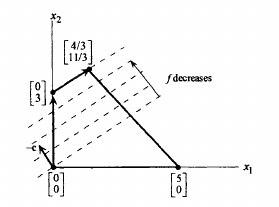
\includegraphics[scale=0.7]{ejemplo}
	\caption{Dibujo del ejemplo}
\end{figure}
\end{example}

\section{Algoritmo del Símplex}
\begin{itemize}
\item Inicialización: encontrar un punto extremo $\overline{x}$ con base $B$.
\item Iteraciones: Calcular $c'_N-c'_B B^{-1}N\equiv c'_N-z_N\equiv \overline{c}_N$. Si este vector es no negativo, paramos(la solución $\overline{x}$ es óptima). En caso contrario, $\exists j\mid c_j-c_B B^{-1}a_j<0$ (si hubiera más de un negativo, elegir el de mayor valor absoluto). Si $y_j=B^{-1}a_j\leq 0$ el problema no tiene mínimo (el mínimo sería $-\infty$). Si $y_{ij}\not\leq 0$ comenzar nuevamente las iteraciones tomando como punto extremo en la inicialización $\hat{x}=\overline{x}+\frac{\overline{b}_r}{y_{rj}}d_j$, siendo $\frac{\overline{b_r}}{y_{rj}}=\min\{\frac{\overline{b_i}}{y_{ij}}:y_{ij}>0\}$, $\overline{b}=B^{-1}b$, $y_j=B^{-1}a_j$, $d_j=\begin{pmatrix}
-y_j\\
e_j
\end{pmatrix}$,
siendo la nueva base la resultante de eliminar la columna $a_r$ de $B$ y en su lugar introducir la columna $a_j$.
\end{itemize}
Este algoritmo tiene el problema de determinar el extremo inicial. Para ello usamos el siguiente método.
\subsection{Método de M-grande}
Consiste en utilizar un problema auxiliar $(P_m)$.
\begin{align*}
 \min\ & c'x+M1^t x_h\qquad \equiv &\min c'x+M\sum_{i=1}^m x_{h_i}\\
&sa:\ Ax+Ix_h=b              & A_1x+ x_{h_1}=b_1 \\
& x\geq 0, x_h\in R^m_+    & \vdots \\
&                          & A_m+ x_{h_m}=b_m
\end{align*}
Donde $A_i$ representa la fila $i$ de la matriz $A$ y $M$ es una constante lo bastante grande (podemos considerar $M=\infty$).  En $P_m$ hay una base obvia $B=[\text{columnas de }x_h]=I$ y $B^{-1}=I\Rightarrow B^{-1}b\geq 0$ si $b\geq 0$. Esto permite aplicar el algoritmo del simplex a $P_m$ para hallar su solución óptima $x^*$. 

Si en $x^*$ hay alguna variable $x^*_{h_i}\neq 0$ para algún $i$, en el objetivo aparece $Mx^*_{h_i}$. Tenemos que $c'x<c'x^*$ para cualquier $x\in P$ (poliedro original), por lo que $P=\emptyset$, porque de haberlo el algoritmo habría encontrado uno más pequeño.  Si $x^*$ es tal que $x^*_h=0$, entonces $x^*$ es solución del problema original $(PL)$. 

\subsection{Forma tabular del algoritmo del símplex}

\begin{align*}
\min & c'x [B N]\\
& Ax=b\\
&x\geq 0
\end{align*}
\begin{tabular}{|c|c| c| c|c|}
\hline
 & & $c'_B$ & $c'_N$ & \\
 \hline
 $x_B$ & $c_B$ & $B$ & $N$ & $b$\\
 \hline

\end{tabular}$\underset{B^{-1},\overline{b}B^{-1}b\geq 0}{\Longrightarrow}$
\begin{tabular}{|c|c| c| c|c|}
\hline
 & & $c'_B$ & $c'_N$ & \\
 \hline
 $x_B$ & $B^{-1}B=I$ & $B^{-1}N=Y$ & $N$ & $\overline{b}$\\
 \hline

\end{tabular}
Apliquemos esto al ejemplo anterior.
\begin{align*}
\min &x_1-3x_2\\
sa & -x_1+2x_2+x_3 \quad = 6\\
   & x_1+x_2 \qquad +x_4 = 5\\
   &x_1,x_2,x_3,x_4\geq 0
\end{align*}
\begin{tabular}{|c|c| c c| c c|c|}
\hline
 &            & $1$ & $-3$ & $0$ & $0$ & $b$  \\
 \hline
 $x_3$ & $0$ & $-1$ & $2$ &   $1$ &   $0$ & $6$\\
  $x_4$ & $0$ & $1$ & $1$ &    $0$ &  $1$ & $5$\\
 \hline
 &            & $1$ & $\boxed{-3}$ & $0$ & $0$ & \\
 \hline

\end{tabular}
Hemos señalado el elemento no positivo. \\

LA EXPLICACIÓN DE CÓMO PASAR DE UNA MATRIZ A OTRA ESTÁ MAL

La fila inferior se obtiene de la siguiente forma. Llamamos $B$ y $N$ respectivamente a las matrices cuadradas que se observan. Sobre cada una de ellas hay un vector, que llamaremos $c_B$ y $c_N$ en cada caso. Llamamos además $v_0$ y $v_1$ a los dos primeros vectores columna ($v_0$ representa los valores de las variables $v_1$ es la primera columna de $B$). Para conseguir el vector bajo $B$ hacemos $c_B-v_1 B$. Análogamente, para el otro vector hacemos $c_N-v_2 N$. Tenemos que $y_2$ es la segunda columna de la matriz $B$. A partir de eso calculamos $\min\{\frac{6}{2}, \frac{5}{1}\}=3$. Este mínimo corresponde a la segunda columna de $B$. Ahora nos interesa que la columna $\begin{vmatrix}
1\\
0
\end{vmatrix}$ aparezca en el lugar de la columna $\begin{vmatrix}
2\\
1
\end{vmatrix}$. Para ello, debemos realizar operaciones por filas. En este caso, basta hacer $\frac{1}{2}F_1$ y a continuación $F_2-F_1$. Además tenemos que sustituir el $x_3$ (por haber eliminado la columna $\begin{vmatrix}
1\\
0
\end{vmatrix}$, que es $v_3$) por el $x_2$ (por corresponderse el mínimo con la segunda columna de $B$). Resultando la tabla siguiente

\begin{tabular}{|c|c| c c| c c|c|}
\hline
 &            & $1$ & $-3$ & $0$ & $0$ & $b$  \\
 \hline
 $x_2$ & $-3$ & $-\frac{1}{2}$ & $1$ &   $\frac{1}{2}$ &   $0$ & $3$\\
  $x_4$ & $0$ & $\frac{3}{2}$ & $0$ &    $-\frac{1}{2}$ &  $1$ & $2$\\
 \hline
 &            & $\boxed{-\frac{1}{2}}$ & $0$ & $\frac{3}{2}$ & $0$ & \\
 \hline

\end{tabular}\

Ahora operamos igual que antes tenemos que el mínimo es $\frac{4}{3}$, y deberíamos seguir así sucesivamente.



% Capítulo 4
\chapter{Dualidad en programación lineal}
\section{Introducción}
A cada problema de programación lineal

\begin{center}
\begin{tabular}{cccccc}
(P) & $\min$ & $c_1'x_1$ & $+c_2'x_2$   & $+c_3'x_3$\\
(u') & sa: & $A_{11}x_1$ & $+A_{12}x_2$ & $+ A_{13}x_3$ & $≥ b_1$\\
(v') &     & $A_{21}x_1$ & $+A_{22}x_2$ & $+ A_{23}x_3$ & $≤ b_2$\\
(w') &     & $A_{31}x_1$ & $+A_{32}x_2$ & $+ A_{33}x_3$ & $= b_3$\\
     &     &       $x_1$ &              &               & $≥ 0$\\
     &     &             &      $x_2$   &               & $≤ 0$\\
     &     &             &              &         $x_3$ & libre
\end{tabular}
\end{center}
al que llamaremos primal (P) y donde $x_1, x_2$ y $x_3$ son vectores de variables de decisión, le vamos a asociar otro problema de programacion lineal al que llamaremos dual (D) dado por las siguiente transformación:

\begin{center}
\begin{tabular}{cccccc}
(D) & $\max$ & $u'b_1$ & $+v'x_2$ & $+w'x_3$\\
    & sa: & $u'A_{11}$ & $+v'A_{12}$ & $+w'A_{13}$ & $≤ c_1'$\\
    &     & $u'A_{21}$ & $+v'A_{22}$ & $+w'A_{23}$ & $≥ c_2'$\\
    &     & $u'A_{31}$ & $+v'A_{32}$ & $+w'A_{33}$ & $= c_3'$\\
    &     &       $u$  &             &             & $≥ 0$\\
    &     &            &      $v$    &             & $≤ 0$\\
    &     &            &             &      $w$    & libre
\end{tabular}
\end{center}

La transformacón que lleva (P) en (D) crea por cada restricción de (P) una variable de decisión en (D) y por cada variable de decisión en (P) una restricción en (D) de a forma que se indica en la siguiente tabla:

\begin{center}
\begin{tabular}{|c|c|}
\hline
	$\min$ & $\max$\\
\hline
	restriccion ≥ & variable ≥ 0\\
\hline
	restricción ≤ & variable ≤ 0\\
\hline
	restricción = & variable libre\\
\hline
	variable ≥ 0 & restricción ≤\\
\hline
	variable ≤ 0 & restricción ≥\\
\hline
	variable libre & restricción = \\
\hline
\end{tabular}
\end{center}

\begin{example}
Consideramos el problema
\begin{align*}(P)
	\min c'x\\
	\text{sa:} Ax ≥ b\\
	x ≥ 0
\end{align*}
podemos transformarlo en el problema:
\begin{align*}(P')
	\min c'x + 0x_a\\
	\text{sa:} Ax-Ix_a = b\\
	x, x_a ≥ 0 
\end{align*}
y finalmente pasarlo al problema dual
\begin{align*}(D)
	\max u'b\\
	\text{sa:} u'A ≤ c'\\
	u ≥ 0
\end{align*}
\end{example}

\begin{theorem}[Teorema de dualidad débil]
Para todo $x \in X$ y $u \in U$, donde $X = \{x \in \R^n : Ax ≥ b, x ≥ 0\}$ y $U = \{ u \in \R^m  u'A ≤ c', u ≥ 0 \}$, se verifica que $c'x ≥ u'b$.
\end{theorem}

\begin{dem}
$\forall u \in U, \forall x \in X$, se tiene que $u'A ≤ c', x ≥ 0$, luego $u'A x ≤ c'x$. Como $u≥0$ y $Ax≥b$, llegamos a que $u'b ≤ u'Ax ≤ c'x$, lo que demuestra el teorema.
\end{dem}

\begin{obser}
En particular, también se verifica que:
\[ \max\limits_{u \in U} u'b ≤ \min\limits_{x\in X} c'x \]
\end{obser}

\begin{coro}
Si $x^* \in X$ y $u^* \in U$ y $c'x^* = (u^*)'b$, entonces $x^*$ y $u^*$ son soluciones óptimas de (P) y (D) respectivamente.
\end{coro}

\begin{dem}
Por la observación anterior, sigue inmediatamente.
\end{dem}

\begin{theorem}[Teorema de dualidad fuerte]
Si $X \neq \emptyset$ y $U \neq \emptyset$, entonces existen $x^*$ y $u^*$ soluciones óptimas de (P) y (D) respectivamente. Además, $c'x^* = (u^*)'b$.
\end{theorem}

\begin{dem}
Como $U \neq \emptyset$, existe algún punto $\overline{u} \in U$. Entonces $\forall x \in X$, $x'c ≥ \overline{u}'b$. Por tanto (P) no puede decrecer a $-\infty$ y esto indica que debe haber una solucion en un punto extremo $x^* \in X$, determinado por una base $B$. Así que:
\[ x^* = \begin{pmatrix}B^{-1} b \\ 0\end{pmatrix}, \qquad B^{-1}b ≥ 0 \]

Veamos ahora que $(u^*)' = c_B'B^{-1}$ es la solución óptima de (D). Es decir, hay que ver que (1) $(u^*)' \in U$ y (2) $(u^*)'b = c'x^*$. Vemos que:
\[ (u^*)'A ≤ c' \equiv (u^*)' (B \ N) ≤ (c_B' \ c_N') \]
Luego:
\[ (u^*)'B ≤ c_B' \equiv c_B'B^{-1}B ≤ c_B \equiv c_B' ≤ c_B'\]
\[ (u^*)'N ≤ c_N' \equiv c_B'B^{-1}N ≤ c_N' \equiv c_N' - c_B'B^{-1}N ≥ 0\]
Como las ecuaciones del miembro derecho se cumplen, llegamos a que $(u^*)'A ≤ c'$, lo que demuestra (1). Por otro lado, dado que $x^*$ es solución óptimma de (P) entonces las cotas reducidas de las variables asociadas a $x_a$ en $Ax - I x_a = b$ deben ser no negativas. Para cualquier columna $a \in A$ o $-e_j \in -I$, se tiene que:
\[ c_a - c_B' B^{-1} a ≥ 0 \]
\[ c_{e_j} - c_B' B^{-1}(-e_j) ≥ 0 \equiv  c_B'B^{-1}(-e_j) ≥ 0 \equiv c_B'B^{-1}e_j = (u^*)'e_j ≥ 0 \]
para todo $j$, luego todas las columnas de $c_B'B^{-1}$ son no negativas, luego $u^* ≥ 0$. Por último:
\[ (u^*)'b = c_B'B^{-1}b = \begin{pmatrix}c_B' & c_N'\end{pmatrix}\begin{pmatrix}B^{-1}b\\0\end{pmatrix} = c'x^* \]
\end{dem}

\begin{lema}
El sistema
\begin{equation*}\label{sistema1}\begin{cases}
	Ax - tb ≥ 0\\
	-u'A + tc' ≥ 0\\
	u'b - c'x ≥ 0
\end{cases}\end{equation*}
admite una solucion $(x_0,u_0,t_0) ≥ 0$ y verificando
\begin{equation*}\label{sistema2}\begin{cases}
	Ax_0 - t_0b +u_0     > 0\\
	-u'_0A + t_0c' + x_0  > 0\\
	u'_0b - c'x_0 + t_0 > 0
\end{cases}\end{equation*}
\end{lema}

\begin{dem}
Basta ver que la matriz del sistema es antisimétrica:
\[ \begin{pmatrix}
	0  &  A  & -b\\
	-A' &  0  & c\\
	b'& -c'  & 0 
\end{pmatrix}\begin{pmatrix}
	u\\x\\t
\end{pmatrix} ≥ 0 \]
\end{dem}

\begin{theorem}[Teorema de dualidad más fuerte de Gale]
Dados (P) y (D) entonces uno y sólo uno de los siguientes casos son ciertos:
\begin{enumerate}
	\item Ambos problemas tienen soluciones óptimas y sus valores coinciden.
	\item Un problema es infactible y el otro tiene solución ilimitada.
	\item Los dos problemas son infactibles.
\end{enumerate}
\end{theorem}

\begin{dem} Consideramos la solución $(x_0,u_0,t_0)$ del sistema del lema anterior. Distinguimos 2 casos:
\begin{enumerate}
	\item $t_0 > 0$. Consideramos $x^* = \frac{x_0}{t_0}$, $u^* = \frac{u_0}{t_0}$ y $t^* = 1$. $(x^*,u^*,t^*)$ sigue siendo solucion del sistema homogéneo. Es decir:
\[\begin{cases}
	Ax^* - b ≥ 0\\
	-(u^*)'A + c' ≥ 0\\
	(u^*)'b - c'x^* ≥ 0
\end{cases}\]
Por lo tanto:
\[\begin{cases}
	Ax^* ≥ b & \Rightarrow x^* \in X\\
	(u^*)'A ≤ c' & \Rightarrow u^* \in U\\
	(u^*)'b ≥ c'x^* & \Rightarrow c'x^* = (u^*)'b
\end{cases}\]
Es decir, $(x^*,u^*)$ es solución óptima de (P) y (D) respectivamente.
	\item $t_0=0$. Se tiene:
\[\begin{cases}
	Ax_0 ≥ 0\\
	-(u_0)'A  ≥ 0\\
	(u_0)'b - c'x^* > 0
\end{cases}\]
	Podemos poner mayor estricto en la última ecuación porque $(u_0)'b-c'x^*+t_0 > 0$.
	\begin{enumerate}
	\item Supongamos que existe $\overline{x} \in X$ y $\overline{u} \in U$, de manera que:
	\[\begin{cases}
		A\overline{x} ≥ b & \overline{x} ≥ 0\\
		\overline{u}'A ≤ c' & \overline{u} ≥ 0
	\end{cases}\]
	Combinando las desigualdades, obtenemos que
	\[ \begin{cases}Ax_0 ≥ 0\\\overline{u} ≥ 0\end{cases} \Rightarrow u'Ax_0≥0 \]
	\[ \begin{cases}\overline{u}A ≤ c'\\x_0 ≥ u'Ax_0 ≤ c'x_0 \end{cases} \Rightarrow u'Ax_0≤c'x_0 \]
	Luego $c'x_0 ≥ 0$. Por otro lado:
	\[ \begin{cases}A\overline{x} ≥ b\\u_0 ≥ 0\end{cases} \Rightarrow u_0'A\overline{x}≥u_0'b \]
	\[ \begin{cases}u'A ≤ 0\\\overline{x} ≥ 0 \end{cases} \Rightarrow 0 ≤ u_0'Ax_0 \]
	Luego $u_0'b ≥ 0$. Pero entonces $c'x_0 ≥ 0 ≥ u_0' b$. con o que llegamos a una contradición si además tenemos en cuenta que $c'x_0 \neq u_0' b$ por la tercera ecuación del sistema.
	
	\item Supongamos que $\overline{x}$ es solución de $P$ y $U = \emptyset$. Tenemos lo siguiente
	\[ \begin{cases}A_0 > 0 \\ -u_0'A ≥ 0 \\ u_0'b-c'x_0 > 0 \\ u_0 ≥ 0, _0 ≥ 0\\ A\overline{x} ≥ b,\overline{x}≥ 0\end{cases} \]
	Vemos que:
	\[ A(\overline{x} + λx_0) = A\overline{x} + λ A x_0 ≥ b \quad \forall λ\]
	Como $\overline{x} + λ x_0 ≥ 0$, $\overline{x} + λ x_0 \in X$ para todo $λ > 0$. Además $c'(\overline{x} + λ x_0) = c'\overline{x} + λ c' x_0$ pero veremos que $c'x_0 < 0$ puesto que
	\[ \begin{cases}u_0'A ≤ 0\\\overline{x} ≥ 0\end{cases} \Rightarrow \underset{≥0}{u_0'}\underset{≥b}{A\overline{x}} ≤ 0 \Rightarrow \begin{cases}u_0'b ≤ u_0'A\overline{x} ≤ 0\\u_0'b > c'x_0\end{cases} \Rightarrow c'x_0 < 0\]
	Pero entonces $c'(\overline{x} + λ x_0) \to -\infty$ cuando $λ \to \infty$. Esto es que no puede darse solucion únicamente de un problema y, por descarte, el último caso es que ninguno tenga solución.
	\end{enumerate}
\end{enumerate}
\end{dem}

\begin{theorem}[Teorema de holgura complementaria fuerte]
Si $X \neq \emptyset$ y $U \neq \emptyset$, existen $(\overline{x},\overline{u})$ óptimos de (P) y (D) tales que:
\[ A\overline{x} -b + \overline{u} > 0\]
\[ -\overline{u}A + c' +\overline{x}' > 0\]
\end{theorem}

\begin{dem}
Estamos en el caso 1 del teorema anterior y, por tanto, $t_0 > 0$. Consideramos $\overline{x} = \frac{x_0}{t_0}$, $\overline{u}=\frac{u_0}{t_0}$ y $\overline{t} = 1$. $(\overline{x},\overline{u},\overline{t})$ es solución del sistema \eqref{sistema1} y cumple (evaluando en \eqref{sistema2}):
\[ A\overline{x} -b + \overline{u} > 0\]
\[ -\overline{u}A + c' +\overline{x}' > 0\]
\end{dem}

\begin{theorem}[Otro teorema de holgura complementaria] Sean $x^*$, $u^*$ soluciones factiables de P y D, respectivamente. Entonces $x^*$ y $u^*$ son soluciones óptimas si y sólo si $u^*(Ax^*-b)=0$, $(u'^{*} A-c')x^*=0$.
\end{theorem}
\begin{dem}
\[
\begin{cases}
u'^* A x^* = u'^*b \\
u'^*A x^* = c'x^* 
\end{cases}
\quad c'x^* = u'^*b \Rightarrow \text{$x^*$ es óptima en P y $u^*$ en D}
\]
Recíprocramente, si $c'x^*=u'^*b$. Consideramos el producto, donde cada miembro es $\geq 0$.
\[
u'^*(Ax^*-b)\geq 0
\]
Veamos que $\not >$. Supongamos lo contrario. ($(u^*A) \leq c'$ por ser solución factible del dual):
\[
u'^*Ax^* > u'^* b \Rightarrow c'x^* \geq u'^*Ab>u'^*b
\]
Lo cual es un absurdo. Análogamente deducimos que $(u'^*A-c')x^* \leq 0$. Si la desigualdad fuera estricta llegaríamos al mismo absurdo que en el caso anterior usando que, como $Ax^* \geq b$.
\end{dem}
\section{Análisis de postoptimalidad}
Dado un problema $(P)$ $\min c'x$, $Ax=b$, $x\geq 0$. Considero un vector $d\in\R^n$ y la familia de problemas: $P(\Delta)$: $\min c'x + \Delta d'x$, $Ax=b$, $x\geq 0$. Observemos que $P=P(0)$. Supongamos que B es una base asociada a una solución óptima de $x^*(0)$. Es decir, $x^*(0)=[B^{-1}b 0]' \geq 0$. Queremos determinar el rango de valores de $\Delta$ que mantienen a $x^*(0)$ como solución óptima de $P(\Delta)$. La condición que ertifica que B es una base óptima son:
\begin{itemize}
\item $B^{-1}b \geq 0$.
\item $\overline{c_R}'(0)_N  = \overline{c}'_N = c'_N - c_N'B^{-1}N \geq 0$. 
\end{itemize}
Las condiciones en $P(\Delta)$. 
\begin{itemize}
\item $B^{-1}b \geq 0$.
\item $\overline{c_R}'_N = (c -\Delta d)'_N- (c+\Delta d)'_B B^{-1}N = \overline{c_R}'(0)_N  + \Delta (d_N'-d'_BB^{-1}N) =  \overline{c_R}'(0)_N + \Delta \overline{d}_N\geq 0$. 
\end{itemize}
Para una componente genérica $j\in \mathbb{N}$ se tiene que $\overline{c}_j+\Delta d_j\geq 0$. Entonces:
\[
\begin{cases}
-\frac{\overline{c}_j}{\overline{d}_j} \geq \Delta & si \quad \overline{d}_j <0\\
-\frac{\overline{c}_j}{\overline{d}_j} \leq \Delta & si \quad \overline{d}_j >0
\end{cases}
\Rightarrow \max_{j:\overline{d}_j >0}-\frac{\overline{c}_j}{\overline{d}_j} \leq \Delta \leq \min_{j:\overline{d}_j <0}-\frac{\overline{c}_j}{\overline{d}_j}
\]

\section{Análisis de las variaciones en términos independientes}

Sea $z(0)= \min c'x$ sujeto a $Ax=b, x\geq 0$. Queremos estudiar que pasa si elegimos $g\in\R^m$ y construimos el problema
\begin{align*}
z(\Delta)=\min c'x\\
sa: Ax=b+\Delta g\\
\Delta\in\R
\end{align*}
Si $B$ es una base asociada a la solución óptima de $z(0)$, ¿cuál es el rango de $\Delta$ que mantiene $B$ óptima? Las condiciones para que sea óptima son:
\begin{enumerate}
\item Condición de optimalidad. \[\overline{c}_N=c'_N-c'_B B^{-1}N\geq 0.\]
En $z(\Delta)$, teniendo en cuenta que no cambia la función ni las columnas de $A$, esta condición es
\[\overline{c}_N=c'_N-c'_B B^{-1}N\geq 0\] si $\overline{c}_N\geq 0$, que lo es. 
\item Factibilidad. En $z(0)$ es $B^{-1}b=\overline{b}\geq 0$. En $z(\Delta)$ es 
\[B^{-1}b(\Delta)=B^{-1}(b+\Delta  g)=B^{-1}b+\Delta B^{-1}g=\overline{b}+\overline{g}\geq 0\]
Tomemos un índice $i$ arbitrario.

\[\overline{b}_i+\Delta\overline{g}_i\geq 0\ \forall i=1,\dots, m\Leftrightarrow -\Delta\overline{g}_i\leq\overline{b}_i\]
Si $g_i<0$: $\Delta\leq\frac{\overline{b}_i}{-\overline{g}_i}$.\\
Si $g_i>0$: $\Delta\geq\frac{-\overline{b}_i}{\overline{g}_i}$.\\
Luego
\[\max_{i, g_i>0}\{\frac{-\overline{b}_i}{\overline{g}_i}\}\leq\Delta \leq \min_{i,g_i<0}\{\frac{-\overline{b}_i}{\overline{g}_i}\}\]
\end{enumerate}
\begin{example}
\begin{align*}
\min & -2x_1-x_2 &\\
sa: & x_1+x_2 &\leq 5\\
    & -x_1+x_2 & =0\\
    & 6x_1+2x_2 & \leq 21\\
    & x_1,x_2 & \geq 0
\end{align*}
Pongamos $g'=(0,0,1)$. La báse óptima para $x_1,x_2,x_4$ de este problema era $B=[a_1\ a_2\ a_4]$. Imponemos $B^{-1}(b+\Delta g)\geq 0$ y despejamos $\Delta$ Obtenemos
\[
\begin{pmatrix}
\frac{11}{4}\\
\frac{9}{4}\\
\frac{1}{2}
\end{pmatrix}+\Delta\begin{pmatrix}
\frac{1}{4}\\
\frac{-1}{4}\\
\frac{1}{2}
\end{pmatrix}\geq 0
\]
Por lo tanto $\Delta\in [-1,9]$. Esto quiere decir que $B$ es óptima para $b_3\in[20,30]$. La solución $x(\Delta)=B^{-1}b(\Delta)$ en cada caso será distinta, pero la base será la misma.
\end{example}

\section{Añadir una nueva variable $x_{n+1}$ a un problema}
Pasamos del problema $(P)$
\begin{align*}
\min\ & c'x\\
sa:\ & Ax=b\\
 & x\geq 0
\end{align*}
al problema $(P')$
\begin{align*}
\min\ & c'x+c_{n+1}x_{n+1}\\
sa:\ & [A|a_{n+1}]\begin{bmatrix}
x\\
x_{n+1}
\end{bmatrix}=b\\
 &  x,x_{n+1}\geq 0
\end{align*}
Dada $B$ una base óptima en $(P)$ queremos determinar una condición para que sea óptima en $(P')$. Las condiciones para $(P')$ son:
\begin{enumerate}
\item Factibilidad, que es la misma que en $(P)$, $B^{-1}b\geq 0$. 
\item Optimalidad. En $(P)$ \[\overline{c}_N=c'_N-c'_B B^{-1}N\geq 0.\]
En $(P')$
\[\overline{c}_N(P')=(c'_N, c_{n+1})-c'_B B^{-1}[N| a_{n+1}]\geq 0\]
Esto es equivalente a que se cumplan al mismo tiempo
\[\overline{c}_N=c'_N-c'_B B^{-1}N\geq 0,\]
que ya la teníamos, y 
\[c_{n+1}-c'_B B^{-1} a_{n+1}\geq 0.\] Esta sería la condición que buscábamos.

\end{enumerate}

\section{Añadir una restricción}
Partimos de nuevo del problema $(P)$ anterior y lo llevamos al problema $(P_q)$
\begin{align*}
\min\ & c'x\\
sa:\  & Ax=b\\
& a'_q x\leq b_q\\
 & x, x_q\geq 0
\end{align*}
Lo escribimos en forma estándar
\begin{align*}
\min\ & c'x\\
sa:\  & Ax=b\\
& a'_q x+h_q= b_q\\
 & x, x_q, h_q\geq 0
\end{align*}
Suponemos que $B$ es una base óptima en $(P)$ y queremos analizar la solución de $(P_q)$. Es decir, $x=\begin{bmatrix}
B^{-1}b\\
0\end{bmatrix}$, $h_q=b_q-(a_q)_B B^{-1}B$.  Evaluamos esta solución en el problema reordenando las columnas de $a_q$.
\[ [(a_q)_B, (a_q)_N]\begin{bmatrix}
B^{-1}b\\
0\end{bmatrix} +h_q=b_q.\] Hay que comprobar que $h_q\geq 0$ para que tenga sentido. La base asociada a esta solución es
\[ B_q=\begin{bmatrix}
B & 0\\
(a_q)_B & 1
\end{bmatrix}.\] La última columna proviene de haber añadido $h_q$. Su inversa tiene la siguiente forma:
\[ B_q^{-1}=\begin{bmatrix}
B^{-1} & 0\\
\alpha & 1
\end{bmatrix},\] con $\alpha$ tal que $(a'_q)_B B^{-1} +\alpha=0$. Es decir, $\alpha=-(a'_q)_B B^{-1}$. Queda pues, finalmente así la inversa (comprobarlo)
\[ B_q^{-1}=\begin{bmatrix}
B^{-1} & 0\\
-(a'_q)_B B^{-1} & 1
\end{bmatrix}.\]
Para que esta solución sea óptima 
\begin{enumerate}
\item $B_q^{-1}\begin{bmatrix}
b\\
b_q
\end{bmatrix}\geq 0$. Esto es equivalente a $\begin{bmatrix}
B^{-1} & 0\\
-(a'_q)_B B^{-1} & 1
\end{bmatrix}\begin{bmatrix}
b\\
b_q
\end{bmatrix}=\begin{bmatrix}
B^{-1}b\\
-(a'_q)_B B^{-1}+b_q
\end{bmatrix}\geq 0$. Observamos que la única condición nueva es $-(a'_q)_B B^{-1}+b_q\geq 0$.
\item $\overline{c}_N(P_q)=c'_N-(c'_B,0)B_q^{-1}\begin{bmatrix}
N\\
(a'_q)_N
\end{bmatrix}\geq 0$. Esto es equivalente a $c'_N-[c'_B B_q^{-1} N + 0]=\overline{c}_N\geq 0$.
\end{enumerate}

\begin{example}
Añadimos al ejemplo anterior la restricción $x_1+x_2\leq 4$ y lo escribimos en forma estándar añadiendo $x_3,x_4,x_5,x_6$.
\begin{align*}
\min & -2x_1-x_2 &\\
sa: & x_1+x_2 +x_3 &= 5\\
    & -x_1+x_2 +x_4 & =0\\
    & 6x_1+2x_2  +x_4 & = 21\\
    & x_1+x_2 +x_6  & = 4\\
    & x_1,x_2,x_3,x_4,x_5,x_6 & \geq 0
\end{align*}
Obsérvese que hemos añadido $x_4$ aunque ya teníamos una igualdad en la segunda restricción. Esto no importa porque la solución puede dar $x_4=0$. En este problema $a'_q=(1,1,0,0,0)$, $b_q=4$ y $B_6=[a_1\ a_2\ a_4\ a_6]$ (la de antes añadiendo $a_6$). Para que sea óptima $-(a'_q)_B B^{-1}+b_q\geq 0$. Si operamos nos da $-\frac{13}{4}\not\geq 0$, por lo que no es óptima. Tendríamos entonces
\[ B_q^{-1}\begin{bmatrix}
5\\
0\\
21\\
4
\end{bmatrix}=\begin{bmatrix}
\frac{11}{4}\\
\frac{9}{4}\\
\frac{1}{2	}\\
-\frac{13}{4}
\end{bmatrix}\]
Como tenemos un elemento negativo, usaríamos el método del símplex dual.
\end{example}

\section{Precios Sombra}
Definimos 
\begin{align*}
f:\R^m\longrightarrow \R & & &\\
 f(b) = & \min\ & c'x\\
                                &sa:\  & Ax=b\\
       							& & x\geq 0
\end{align*}
Queremos derivar esta función. Supongamos en este problema que las bases factibles son $B_1,\dots, B_r$. Consideramos el problema dual que verifica
\begin{align*}
 f(b) = & \min\ & c'x\quad  & =\max\ u'b \quad  = \max\{c'_{B_1}b,\dots, c'_{B_r}b\}\\
        &sa:\   Ax=b       &sa:\ & u'A\leq b\\
        &  x\geq 0         & & u\in\R^m 
\end{align*}
Llamamos $u_i=c'_{B_i}$. Entonces, $f(b)=\max_{1\leq i\leq r}u_i'B=u'_k b$. Ahora derivamos
\[\frac{\partial f}{\partial u_i}=\frac{\partial }{\partial b_i}\left(\sum_{j=1}^m u_{kj}b_j\right)=u_{ki}\]
Hemos llegado a la solución óptima del dual en su variable $i$-ésima. 
\begin{example}
$g'(0,0,1)=e'_3$. Teníamos que $z(\Delta)$ al variar $b_3\in [20,30]$ mntiene la base óptima.
\begin{gather*}
f(\Delta)= z(\Delta)=c'_B B^{-1}b(\Delta)=c'_B B^{-1}(b+\Delta e_3)=\\
c'_B B^{-1} b +\Delta c'_B B^{-1} e_3 =\frac{31}{4}-\frac{1}{4}\Delta
\end{gather*}
Luego $\frac{\partial z}{\partial\Delta}=-\frac{1}{4}$. Si quisiéramos utilizar el resultado anterior, tendríamos que obtener la solución óptima y multiplicar por $e_3$ (quedarnos con la tercera componente). La solución óptima del dual es
\[(u^*)'=c'_B B^{-1}=[-2\ -1\ 0]B^{-1}=[-\frac{1}{2}\ 0\ -\frac{1}{4}]\]
Por lo tanto. $\frac{\partial z}{\partial\Delta}=\frac{\partial z}{\partial b_3}=u^*_3=\frac{1}{4}$.
\end{example}



\end{document}
